\chapter{The Wave Equation}

\section{Exercises}

\exercise{1.4}{
	Given positive constants A, a, and b:
	\begin{flalign*}
		\Psi(x,0) =
		\begin{cases}
			A(x/a),       & \text{if}\ 0 \leq x \leq a, \\
			A(b-x)/(b-a), & \text{if } a \leq x \leq b  \\ 0 &
			   \text{otherwise}
		\end{cases}
	\end{flalign*}

	\begin{itemize}
		\item Normalize $\Psi$.
		      \begin{flalign*}
			      \int_{-\infty}^\infty |\Psi(x,t)|^2 ~dx = 1
			      \\
			      A^2\left( \int_0^a \frac{x^2}{a^2} ~dx +
			      \int_a^b \frac{(b-x)^2}{(b-a)^2} ~dx \right) & =
			      1                                                \\
			      A^2\left( \frac{a}{3} + \frac{b-a}{3} \right)
			                                                   & =
			      1 \implies A = \sqrt[2]{\frac{3}{b}}             \\
			      \Psi(x,0) =
			      \begin{cases}
				      \sqrt[2]{\frac{3}{b}}(x/a),       &
				      \text{if}\ 0 \leq x \leq a,         \\
				      \sqrt[2]{\frac{3}{b}}(b-x)/(b-a), &
				      \text{if } a \leq x \leq b          \\ 0 &
				         \text{otherwise}
			      \end{cases}
		      \end{flalign*}
		\item Where is particle most likely to be found at $t = 0$?
		      Based on plots, you will see it is most likely at
		      position a.
		\item Probablility of finding particle to the left of a? Check
		      with b = a and b = 2a.
		      \begin{flalign*}
			      \int_0^a \left|
			      \sqrt[2]{\frac{3}{b}}(x/a)\right|^2 ~dx \\
			      \int_0^a \frac{3}{b}(x^2/a^2) ~dx =
			      \frac{a}{b}
		      \end{flalign*}
		\item What is the first moment (expected value) of x?
		      \begin{flalign*}
			      \langle x \rangle &=\int_0^b x\Psi(x,t) dx = \int_0^a \sqrt[2]{\frac{3}{b}}(x/a) ~dx + \int_a^b  \sqrt[2]{\frac{3}{b}}(b-x)/(b-a) ~dx\\
				  &=\frac{b+2a}{4}
		      \end{flalign*}
	\end{itemize}
}

\exercise{1.5MOD}{
	Given positive, real constants A, $\lambda$, $\omega$:
	\begin{flalign*}
		\Psi(x,t) = Ae^{-\lambda|x|-i\omega t}
	\end{flalign*}
	\begin{itemize}
		\item Normalize $\Psi$.
		\begin{flalign*}
			&\int_{-\infty}^{\infty} |\Psi(x,t)|^2 ~dx =  \int_{-\infty}^{\infty} \Psi^* \Psi = 1\\
			&\int_{-\infty}^{\infty} A^2 e^{-2\lambda |x|} e^{-i\omega t}e^{i\omega t} ~dx =1\\
			A^2 &\int_{-\infty}^{\infty} e^{-2\lambda |x|} ~dx =1\\
			A^2 &\left( \int_{-\infty}^{0} e^{-2\lambda \cdot (-x)}~dx + \int_{0}^{\infty} e^{-2\lambda \cdot (x)} \right) = 1\\
			A^2 &\left( \frac{1}{2 \lambda}e^{2 \lambda x} \right)  \Biggr|_{-\infty}^0 - A^2 \left( \frac{1}{2 \lambda}e^{-2 \lambda x} \right)  \Biggr|_{0}^\infty =1\\
			&\frac{A^2}{\lambda} =1 \implies A = \sqrt[2]{\lambda}\\
			\Psi(x,t) &= \sqrt{\lambda}e^{-\lambda|x|-i\omega t}\\
			|\Psi(x,t)|^2 &= \Psi^* \Psi = \lambda e^{-\lambda|x|-i\omega t} e^{-\lambda|x|+i\omega t} = \lambda e^{-2 \lambda |x|}
		\end{flalign*}
		\item Find the $n^{th}$ moment.
			\begin{flalign*}
				\langle x^n \rangle &= \int_\mathbb{R}  x^n \lambda e^{-2 \lambda |x|} ~dx\\
				&= \lambda \left(  \int_{-\infty}^0 x^n e^{2 \lambda x} + \int_{0}^\infty x^n e^{-2 \lambda x}\right) ~dx
			\end{flalign*}
			Now note the following is smells like the gamma function, and make substitution of $u = -x$ to change limits (also note that n is positive to extract the alternating negative one):
			\begin{flalign*}
				I_{n_1} = \int_{-\infty}^0 x^n e^{2 \lambda x} ~dx = \int_{\infty}^0 (-u)^n e^{2\lambda (-u)}~(-du) = -\int_{\infty}^0 (-1)^n u^n e^{-2 \lambda u} ~du  = (-1)^n \int_{0}^{\infty} x^n e^{-2 \lambda x} ~dx
			\end{flalign*}
			By using substitution of the type $u = 2 \lambda x$ we get,
			\begin{flalign*}
				I_{n_1} = \frac{(-1)^n}{2\lambda (2\lambda)^n} \int_0^\infty e^{-u}u^n du = \frac{(-1)^n}{(2\lambda)^{n+1}} \Gamma(n+1), ~\Re(n) > -1
			\end{flalign*}
			where the last equation can be used to show the required base case of $I_0=\frac{1}{2\lambda}$. A similar analysis for the second integrand gives us the combined relation
			\begin{flalign*}
				\langle x^n \rangle &= \lambda I_n = \lambda(I_{n_1}+I_{n_2}) \\
				& = \lambda \Biggl( \frac{(-1)^n + 1}{(2\lambda)^{n+1}}\Biggr)\Gamma(n+1)
			\end{flalign*}
			For practical purposes, we see that the first few moments give
			\begin{flalign*}
				\langle x \rangle &= 0\\
				\langle x^2 \rangle &= \frac{2 \lambda}{8 \lambda^3}\Gamma(3) = \frac{1}{2 \lambda^2}\\
				\langle x^3 \rangle &= 0 \\
				\langle x^4 \rangle &= \frac{2 \lambda}{32 \lambda^5}\Gamma(4) = \frac{3}{8 \lambda^4}
			\end{flalign*}
			\item Find standard deviation. Compute probability particle is outside one standard deviation from the mean.
			\begin{flalign*}
				\sigma^2 &= \langle x^2 \rangle - \langle x \rangle^2 \implies \sigma = \frac{1}{\lambda \sqrt{2}}\\
				|\Psi(0\pm \sigma, t)|^2 &= |A|^2e^{-2\lambda \sigma}=\lambda e^{-\sqrt{2}}\\
				P_{outside} &= 1-P_{inside} = 1 - \int_{-\sigma}^{\sigma} |\Psi|^2 ~dx =1 - |A|^2 \int_{-\sigma}^{\sigma} e^{-2 \lambda |x|} ~dx = 2 \lambda \int_{\sigma}^{\infty} e^{-2 \lambda x} ~dx = e^{-\sqrt{2}}
			\end{flalign*}
	\end{itemize}
}

\exercise{1.6}{
	Why can't you do integration-by-parts (IBP) directly in the middle expression of Equation 1.29 -- pull the time derivative over into x, note that $\frac{\partial x}{\partial t}= 0$, and conclude that $\frac{ \langle x \rangle }{dx} = 0$?
	 \\ \\Well, you could but this would not allow us to do IBP over some domain D:
	\begin{flalign*}
		\frac{\partial x|\Psi|^2}{\partial t}=\frac{\partial x}{\partial t}|\Psi|^2+x\frac{\partial |\Psi|^2}{\partial t}=x \frac{\partial |\Psi|^2}{\partial t}\\
		\int_{\partial D} x\frac{\partial |\Psi|^2}{\partial t} dx = \int_{\partial D} \frac{\partial (x|\Psi|^2)}{\partial t} dx \neq (x|\Psi|^2) |_{\partial D}
	\end{flalign*}
}

\exercise{1.7}{
	Calculate $\frac{d\langle p \rangle}{dt}$.\\ \\ By Ehrenfest's theorem, expectation values are goverened by classical laws: $\langle p \rangle = m \langle v \rangle = m\frac{d \langle x \rangle}{dt}$.
	Recall the time derivatives for the conjugate pairs or derive it
	yourself. Also note that interchange of differentiaiton to integration
	(Leibnitz integral rule) implicitly assumes the (wave) function and its first
	partial derivative are continuous in time and space (both) in the open
	neighborhood of $\{x\} \times [a,b]$ for any continuous and differentiable
	functions a, b. Text assumes all partials continuous, and by extent
	differentiable (converse not necessarily true). Second order partials assumed continuous for Clairaut's Theorem, $C^2$, throughout text.
	\begin{flalign*}
		\frac{d\langle p \rangle}{dt} &= -i\hbar \int \pdv{\Psi^* \pderivative{\Psi}{x}}{t}~dx\\
		\frac{\partial \Psi^* \frac{\partial \Psi}{\partial x}}{\partial t}\\
		&=\pdv{\Psi^*}{t}\pdv{\Psi}{x}+\Psi^* \pdv[2]{\Psi}{x}{t}\\
		&=\Bigl(\frac{-i\hbar}{2m}\pdv[2]{\Psi^*}{x}+\frac{iV(x,t)\Psi^*}{\hbar}\Bigr)\pdv{\Psi}{x}+\Psi^*\pdv*{\frac{i \hbar}{2m}\pdv[2]{\Psi}{x}-\frac{iV(x,t)\Psi}{\hbar}}{x}\\
		&= \frac{i \hbar}{2m}\Bigl(\pdv[3]{\Psi}{x}\Psi^*-\pdv[2]{\Psi^*}{x}\pdv{\Psi}{x} \Bigr) + \frac{i}{\hbar} \Bigl(V(x,t)\pdv{\Psi}{x}-\Psi^*\pdv{V(x,t)\Psi}{x}\Bigr)\\
		&= \frac{i \hbar}{2m}\Bigl(\pdv[3]{\Psi}{x}\Psi^*-\pdv[2]{\Psi^*}{x}\pdv{\Psi}{x} \Bigr) + \frac{i}{\hbar} \Bigl(V(x,t)\pdv{\Psi}{x}-\Psi^* V(x,t)\pdv{\Psi}{x}- \Psi^* \pdv{V(x,t)}{x}\Psi\Bigr)\\
		&= \frac{i}{\hbar} \Bigl(|\Psi|^2 \pdv{V(x,t)}{x}\Bigr)\\
	\end{flalign*}
	Whereby we used IBP twice to drop the first term. Accordingly,
	\begin{flalign*}
		\pdv{\langle p \rangle}{t} = -i\hbar \frac{i}{\hbar} \int_{\mathbb{R}} -|\Psi|^2\pdv{V}{x} ~dx = \langle -\pdv{V}{x} \rangle
	\end{flalign*}
	Thus, the time derivative of the expectation value of momentum is equal to the position derivative of the expectation value of potential well V.
}\\

\exercise{1.8}{
	Suppose we add a constant $V_0$ to the potential energy. In classical mechanics, this won't change a thing, but what about in quantum mechanics? 
	Show that the function picks up a time-dependent phase factor. What effect does this have on the expectation value of a dynamic variable?
	\\ \\
	\begin{flalign*}
		\pdv{\Psi}{t} = \frac{i\hbar}{2m}\pdv[2]{\Psi}{x}-\frac{i}{\hbar}V(x,t)\Psi(x,t)
	\end{flalign*}
	Set $\zeta(x,t)$ to the wave function holding potential energy $V(x,t)+V_0$ and rewrite to notice a familiar separable PDE,
	\begin{flalign*}
		\pdv{\zeta}{t} &= \frac{i \hbar}{2m}\pdv[2]{\zeta}{x}-\frac{i}{\hbar}\Bigl(V(x,t)+V_0\Bigr)\zeta\\
		&\implies \frac{i \hbar}{2m}\pdv[2]{\zeta}{x} - \frac{i V \zeta}{\hbar} = \pdv{\zeta}{t}+\frac{iV_0 \zeta}{\hbar}\\
	\end{flalign*}
	We consider the following boundary conditions (BC): $\zeta\left(\infty, t\right) = \zeta \left( -\infty, t \right) =0$. We then proceed with letting $\zeta = X(x)T(t)$. Also, for this course, we are dealing mostly with the time-independent wave equation, such that the potential well is independent of time, $V(x,t)=V(x)$.
	\begin{flalign*}
		\zeta \left(x,t\right) &= X \left(x\right)T\left(t\right)\\
		\zeta\left(\infty,t\right)&=X\left(\infty \right)T\left(t\right)  ~~\forall t \implies c_1 = X(\infty)=0\\
		\zeta\left(-\infty,t\right)&=X\left(-\infty \right)T\left(t\right)  ~~\forall t \implies c_2 = X(-\infty)=0\\
		\frac{i \hbar}{2m}\pdv[2]{XT}{x}-\frac{iV(x) XT}{\hbar} &= \pdv{XT}{t}+\frac{iV_0 XT}{\hbar}\\
		\frac{i \hbar}{2m} X''T-\frac{iV(x) XT}{\hbar} &= XT'+\frac{iV_0 XT}{\hbar}\\
		-\frac{\hbar^2}{2m}\frac{X''}{X} +V(x) &= \frac{T'}{T}i \hbar -V_0\\
		k\frac{X''}{X}+V(x) &= \frac{T'}{T}i \hbar - V_0 = E \text{, up to constant E, now decompose to ODEs}\\
		kX'' &= X(E-V(x)) \text{, stop here as we need potential energy specified, else BC gives trivial solutions} \\
		\frac{T'}{T} &= -i\frac{E+V_0}{\hbar}\\
	\end{flalign*}
	For arbitrary constant C (and thus also $\zeta_0$),
	\begin{flalign*}
		\zeta(x,t) = e^{-\frac{i(E+V_0)t}{\hbar}+C} = \zeta_0 e^{-\frac{i(V_0+E)}{\hbar}t} \\
	\end{flalign*}
	Thus, when plugging this back in to the wave equation (and seeings results from the next chapter!)
	we note the implication: $\Psi(x,t) = \zeta(x,t)e^{\frac{i V_0}{\hbar}t}$. If we substitute into Equation 1.36, then we see that it remains unchanged. 
	We conclude that this has no effect on the expectation value of a dynamical variable, since the extra phase factor cancels out and is independent of position.\\
}

\exercise{1.9MOD}{
	A particle of mass $m$ has the wave function (for positive constants A, a) of $$\Psi(x,t) = Ae^{-a\frac{mx^2}{\hbar}-ait}$$
	\begin{itemize}
		\item Normalize to find A. Watch video on Gaussian integral if stuck on how to derive it.
			\begin{flalign*}
				\int_\mathbb{R} |\Psi(x,t)|^2 ~dx &= \int_\mathbb{R} \Psi^* \Psi ~dx =1\\
				&= A^2 \int_\mathbb{R} e^{-\frac{2amx^2}{\hbar}} ~dx\\
				&= A^2 \sqrt{\frac{\pi \hbar }{2am}} \implies A = \sqrt[4]{\frac{2am}{\pi \hbar}}\\
				\Psi(x,t) &= \sqrt[4]{\frac{2am}{\pi \hbar}} e^{-a\frac{mx^2}{\hbar}-ait}
			\end{flalign*}
		\item For which potential energy function, $V(x)$, is this a solution to Schro's wave equation?
		 	\begin{flalign*}\
				\pdv{\Psi}{t} &= -ia\Psi\\
				\pdv{\Psi}{x} &= -\frac{2amx}{\hbar}\Psi\\
				\pdv[2]{\Psi}{x} &= \frac{-2am}{\hbar}\Bigl(\Psi + x\pdv{\Psi}{x}\Bigr)\\
				&= \frac{-2am}{\hbar} \Bigl( 1 -\frac{ 2amx^2}{\hbar}\Bigr)\\
				i\hbar\pdv{\Psi}{t} &= -\frac{\hbar^2}{2m}\pdv[2]{\Psi}{x}+V(x)\Psi\\
				V(x) &= i\hbar(-ia\Psi)+\frac{\hbar^2}{2m}\Bigl(1-\frac{2amx^2}{\hbar}\Bigr) \Bigl( \frac{-2am}{\hbar}\Bigr)\Psi\\
				& = 2a^2mx^2 \\
		 	\end{flalign*} 
		\item Find the $n^{th}$ moment.\\ \\
			Recall details in problem 1.5 and note $n$ is a positive constant. Here, we split up the integral as was performed then, for negative infinity to 0 then 0 to positive infinity. This simplifies calculation. We set $C = \frac{2am}{\hbar}$ and use $A$ for constant above.
			\begin{flalign*}
				\int_\mathbb{R} x^n|\Psi(x,t)|^2 ~dx &= \int_\mathbb{R} \Psi^* [x^n]\Psi ~dx\\
				& = A^2 \int_\mathbb{R} x^n e^{-Cx^2} ~dx\\
				I_{left} &= \int_{-\infty}^0 x^n e^{-Cx^2} ~dx = (-1)^n\int_0^{\infty} (x^n)e^{-Cx^2}~dx\\
			\end{flalign*}
			From here, you may use substitution of $u = x^2$, then $z = Cu$, to arrive at:
			\begin{flalign*}
				\frac{(-1)^n}{2C^{\frac{n+1}{2}}}\int_{0}^{\infty} e^{-z} z^{\frac{n-1}{2}} ~dz = \frac{(-1)^n}{2C^{\frac{n+1}{2}}}\Gamma \Bigl( \frac{n+1}{2}\Bigr) \\
			\end{flalign*}
			A similar analysis for the positive side results in a similar answer. Combining for the intended integral and substitute back into our original expression:
			\begin{flalign*}
				\langle x^n \rangle &= \frac{A^2((-1)^n+1)}{2C^{\frac{n+1}{2}}}\Gamma \Bigl( \frac{n+1}{2}\Bigr)\\
				\langle x \rangle &= 0\\
				\langle x^2 \rangle &= \frac{1}{2}(2)\sqrt[2]{\frac{2am}{\pi \hbar}} \Biggl(\frac{2am}{\hbar} \Biggr)^{-3/2} \cancelto{\frac{\sqrt{\pi}}{2}}{\Gamma \Bigl( \frac{3}{2} \Bigr)}\\
				&= \frac{\hbar}{4am}
			\end{flalign*}
		\item Find the expression for the $p^{th}$ momentum. Note it gives non-trivial position partials for the first five degrees. 
		 \begin{flalign*}
			\langle p^n \rangle = \int_\mathbb{R} \Psi^* \Bigl(\frac{\hbar}{i}\pdv{}{x}\Bigr)^n \Psi ~dx &= \Bigl(\frac{\hbar}{i}\Bigr)^n \int_\mathbb{R} \Psi^* \pdv[n]{\Psi}{x}\\
			\langle p \rangle &= 0\\
			\langle p^2 \rangle &= am \hbar
		 \end{flalign*}
		\item Find $\sigma_x$ and $\sigma_p$. Is their product consistent with the uncertainty principle?
		 \begin{flalign*}
			\sigma_x = \sqrt{\langle x^2 \rangle - \langle x \rangle } = \frac{\hbar}{4am}\\
			\sigma_p = \sqrt{\langle p^2 \rangle - \langle p \rangle } = \sqrt{am\hbar}\\
			\sigma_p\sigma_x = \frac{\hbar}{2} \geq \frac{\hbar}{2}
		 \end{flalign*}
		 This implies we have a wave function that barely satisifes the uncertainty principle.
	\end{itemize}

}
\exercise{1.11}{
	Imagine a mass particle $m$ and energy $E$ in a potential well $V(x)$ sliding back and forth on a frictionless surface between $a$ and $b$ given in Figure 1.10.
	Classically, the probability of finding particle in range $dx$ is equal to the fraction of time $T$ it takes to get from $a$ to $b$ that it spends on the interval $dx$, and for speed $v(x)$:
	\begin{flalign*}
		\rho(x)dx = \frac{dt}{T} &= \frac{\derivative{t}{x}	dx}{T} = \frac{1}{v(x)T}dx\\
		T &= \int_0^T dt = \int_a^b \frac{1}{v(x)}dx\\
		\implies \rho(x) &= \frac{1}{v(x)T}
	\end{flalign*}
		\begin{itemize}
			\item Use conservation of energy to express speed in terms of potential well and energy.
				\begin{flalign*}
					E = U + K &= V(x) + \frac{mv(x)^2}{2}\\
				\end{flalign*}
			\item Find the probability density for simple harmonic oscillator, $V(x)=\frac{kx^2}{2}$. Check normalization.
				\begin{flalign*}
					v(x) &= \pm \sqrt{\frac{2(E-V(x))}{m}} = \pm \sqrt{\frac{2E-kx^2}{m}}\\
					\rho(x) &= \frac{1}{ \sqrt{\frac{2E-kx^2}{m}} \int_{-A}^{A} \frac{1}{ \sqrt{\frac{2E-kx^2}{m}}} ~dx}\\
					&= \frac{1}{ \sqrt{\frac{2E-kx^2}{m}}\sqrt{\frac{m}{2E}}\int_{-A}^{A}\frac{1}{\sqrt{1-\frac{kx^2}{2E}}}~dx}\\
					&= \frac{1}{ 2\sqrt{1-\frac{kx^2}{2E}}\int_{0}^{A}\frac{1}{\sqrt{1-\frac{kx^2}{2E}}}~dx}\\
				\end{flalign*}
				Now apply a trig substitution to simplify computation; see Paul's online math notes.
				\begin{flalign*}
					x &= \frac{1}{\sqrt{\frac{k}{2E}}}\sin \theta = \sqrt{\frac{2E}{k}} \sin \theta,~\theta \in \left[\frac{-\pi}{2}, \frac{\pi}{2} \right]\\
					\cos^2 \theta &= 1 - \sin^2 \theta = 1 - \frac{k}{2E}x^2 \implies \cos \theta = \sqrt{1-\frac{kx^2}{2E}}\\
					dx &= \sqrt{\frac{2E}{k}}\cos \theta d\theta \\
				\end{flalign*}
				Where we note that for a SHO, the turning points are at the amplitudes $\pm A$ of the oscillation and apply the familiar trigonometric substitution. We drop $\pm$ to focus on the magnitude of $dx$. 
				\begin{flalign*}
					\frac{1}{2\sqrt{1-\frac{kx^2}{2E}}\sqrt{\frac{2E}{k}}\int_{\theta = 0}^{\theta = \sin^{-1} A\sqrt{\frac{k}{2E}}}~d\theta} &= \frac{1}{2\sqrt{1-\frac{kx^2}{2E}}\sqrt{\frac{2E}{k}}\int_{\theta = 0}^{\theta = \sin^{-1} 1}~d\theta}\\
					&= \frac{1}{\pi \sqrt{A^2 - x^2}}\\
					\rho(x) &= 
					\begin{cases}
						\frac{1}{\pi \sqrt{A^2 - x^2}},       & \text{if}\ -A < x < A, \\
						0 & \text{otherwise}
					\end{cases}\\
					\int_{-A}^A \rho(x) ~dx = \frac{2}{\pi}\int_{0}^{A} \frac{1}{\sqrt{A^2 - x^2}} ~dx = \frac{2}{\pi}\sin^{-1}\frac{x}{A} \Biggr|_{0}^A = 1\\
				\end{flalign*}
				\item Find the first and second expected value of position. Find $\sigma_x$. Note that knowing the odd integrand for an even interval yields 0, but can verify with substitution, $u = A^2 - x^2$. It is also helpful to use $x = A \sin \theta$ for the second moment substitution.
				\begin{flalign*}
					\langle x \rangle &= \int_{-A}^{A}\frac{x}{\pi \sqrt{A^2 - x^2}}~dx ~/~ 1 = 0\\
					\langle x^2 \rangle &= \int_{-A}^{A}\frac{x^2}{\pi \sqrt{A^2 - x^2}}~dx ~/~ 1 = \frac{2}{\pi} \Biggl(  \frac{-x \sqrt{A^2-x^2}}{2}+\frac{A^2}{2}\sin^{-1} \frac{x}{A}\Biggr)\Biggr|_{-A}^A = \frac{A^2}{2}\\
					\sigma_x &= \langle x^2 \rangle - \langle x \rangle^2 \implies \sigma_x = \frac{A}{\sqrt{2}}
				\end{flalign*}
				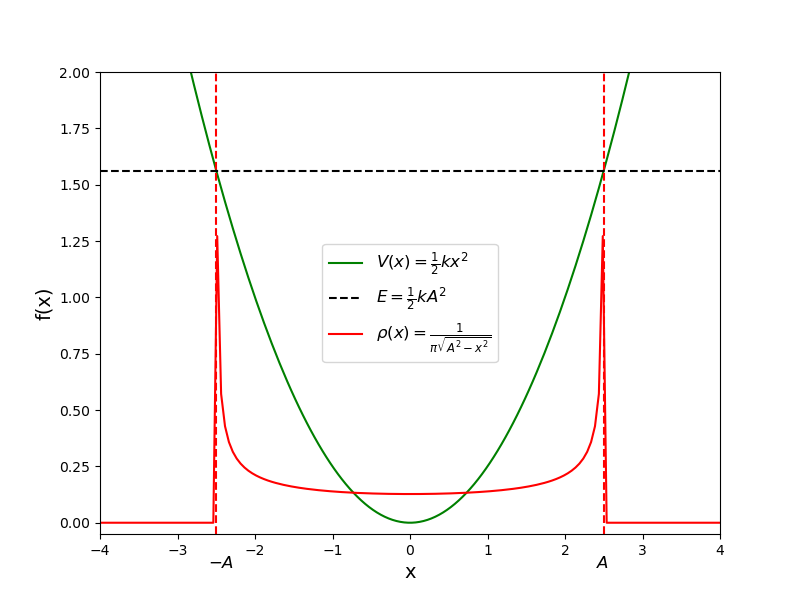
\includegraphics[width=\textwidth]{./chapters/graphs_ch1/1_11_1.png}

		\end{itemize}
}

\exercise{1.12}{
	What if we are interested in finding the momenta ($p=mv$) distribution for the classical harmonic oscillator? 
	\begin{itemize}
		\item Find the classical probability distribution $\rho(p)$; note that $p \in \left[-\sqrt{2mE}, \sqrt{2mE} \right]$.
		As before, we compute total energy and substitute.
		\begin{flalign*}
				E = U+K &= \frac{kx^2}{2}+\frac{mv(x)^2}{2} = \frac{1}{2}kx^2+\frac{p(x)^2}{2m}\\
				\implies x(p) &= \pm \sqrt{\frac{2mE-p^2}{mk}}\\
				dx &= \pm \frac{-p}{mk}\frac{1}{\sqrt{\frac{2mE-p^2}{mk}}}~dp = \mp \frac{p}{mk}\frac{1}{\sqrt{\frac{2mE-p^2}{mk}}}~dp = \mp \frac{p}{mk(2mE-p^2)}~dp\\
				\rho(x(p))dx &= \frac{dt}{T} = \frac{\derivative{t}{x}	dx}{T} = \pm \frac{1}{v(x(p))T}dx = \frac{1}{v(x(p))T}\Bigl(\mp \frac{p}{\sqrt{mk(2mE-p^2)}}~dp \Bigr)\\
				& = \mp \frac{1}{v(p)T}\Bigl(\frac{p}{\sqrt{mk(2mE-p^2)}}~dp \Bigr) = \rho(p)\frac{p}{\sqrt{mk(2mE-p^2)}}~dp\\
				T &= \int_{p(a)}^{p(b)}  \mp \frac{1}{v(p)} \underbrace{\Bigl(\frac{p}{\sqrt{mk(2mE-p^2)}}~dp \Bigr)}_{dx(p)}\\
				\therefore \rho(p) = \frac{1}{v(p)\int_{-\sqrt{2mE}}^{\sqrt{2mE}} \mp \frac{1}{v(p)}\Bigl(\frac{p}{\sqrt{mk(2mE-p^2)}}~dp \Bigr)}
		\end{flalign*}
		Observe $\frac{1}{v(p)} = \frac{dt}{dx(p)}$, and so $\mp C(p)~dp \implies \pm dx(p)$. Recall that the net external force equals the change in momentum of a system divided by the time over which it changes. As the particle moves leftward, the change in distance is negative but the change in momentum is positive,
		 so $p(a) = \sqrt{2mE}$ (i.e., it starts to slow down while gaining momentum in the direction of the net restoring force, which pushes the particle in the opposite direction -- namely, towards equilibrium where force is net zero.) Similarly, the particle reaches the equilibirum point but has gained momentum, moving
		 past this location, with the restoring force growing to act in the opposite direction to slow the particle and return it to equilibirum; thus, the change in momentum is negative, and so $p(b)=-\sqrt{2mE}$. Energy is conserved if the process repeats ad nauseum without any frictional (damping) forces. To change the limits of integration to the form above,
		 simply note that the inverse relationship holds as expressed in the $\mp$ indication of the integrand. We now drop this entirely to focus on the magnitude of change over the range, $dx(p)$. 
		\begin{flalign*}
			\rho(p) &= \frac{1}{v(p)\int_{-\sqrt{2mE}}^{\sqrt{2mE}}\frac{1}{v(p)}\Bigl(\frac{p}{\sqrt{mk(2mE-p^2)}}~dp \Bigr)}\\
			&= \frac{1}{\frac{p}{m}\int_{-\sqrt{2mE}}^{\sqrt{2mE}}\frac{1}{\frac{p}{m}}\Bigl(\frac{p}{\sqrt{mk(2mE-p^2)}}~dp \Bigr)}\\
			&= \frac{1}{\frac{p}{\sqrt{mk}}\int_{-\sqrt{2mE}}^{\sqrt{2mE}}\frac{dp}{\sqrt{2mE-p^2}}}\\
		\end{flalign*}
		Make a trigonometric substitution,
		\begin{flalign*}
			p &= \sqrt{2mE}\sin\theta,~\theta \in \left[\frac{-\pi}{2}, \frac{\pi}{2}\right]\\
			dp &= \sqrt{2mE}\cos\theta\\
			\theta &= \sin^{-1}\frac{p(x)}{\sqrt{2mE}}\\
			p^2 &= 2mE\sin^2\theta \implies 1 - \sin^2\theta = \cos^2\theta = 1 - \frac{p^2}{2mE}\\
			\therefore 2mE\cos^2 \theta &= 2mE - p^2\\
		\end{flalign*}
		Making the substitutions and computing, we see that $\rho(p) = \frac{\sqrt{mk}}{\pi p}$. Also, by using trigonometric substitution,
		 we can show $$\int \rho(x(p))~dx = \int_{-\sqrt{2mE}}^{\sqrt{2mE}}\rho(p)\frac{p}{\sqrt{mk(2mE-p^2)}}~dp = \int_{-\sqrt{2mE}}^{\sqrt{2mE}}\frac{\sqrt{mk}}{\pi p}\frac{p}{\sqrt{mk(2mE-p^2)}}~dp  = 1$$
		\item Calculate $\langle p \rangle$, $\langle p^2 \rangle$, and $\sigma_p$.
		\begin{flalign*}
			\langle p \rangle &= \int_{-\sqrt{2mE}}^{\sqrt{2mE}} p\rho(x(p))~dp =\int_{-\sqrt{2mE}}^{\sqrt{2mE}}p\frac{\sqrt{mk}}{\pi p}\frac{p}{\sqrt{mk(2mE-p^2)}}~dp=0\\
			\langle p^2 \rangle &=  \int_{-\sqrt{2mE}}^{\sqrt{2mE}} p^2\rho(x(p))~dp = \int_{-\sqrt{2mE}}^{\sqrt{2mE}}p^2\frac{\sqrt{mk}}{\pi p}\frac{p}{\sqrt{mk(2mE-p^2)}}~dp=mE\\
			\sigma_p &= \sqrt{\langle p^2 \rangle - \langle p \rangle} = \sqrt{mE}\\
		\end{flalign*}
		\item What is the classical undertainty product $\sigma_x\sigma_p$ for this system? 
		Notice that this product can be as small as you like, classically, simply by sending $E \rightarrow 0$.
		But in quantum mechanics, the energy of a SHO cannot be less than $\hbar\omega/2$, where $\omega = \sqrt{k/m}$ is the classical frequency. In that case what can you say about the uncertainty product?
		Recall $\sigma_x = \frac{A}{\sqrt{2}}$ as found previously.
		\begin{flalign*}
			\sigma_p\sigma_x = A\sqrt{\frac{mE}{2}}
		\end{flalign*}
		Now, for the quantum case, $E \geq \hbar \omega/2$. Therefore,
		\begin{flalign*}
			\sigma_p\sigma_x \geq A \sqrt{\frac{m \frac{\hbar \omega}{2}}{2}} = A\frac{\sqrt{\hbar \omega m}}{2}
		\end{flalign*}
		With a more precisely determined amplitude of oscillation, the more precisely we can determine a particle's position and the less precisely we can determine its momentum.
		Conversely, with a more precisely determined particle frequency, the more precisely we can determine its momentum and the less precisely we can determine its position.\\\\
		Aside: From the de Broglie relation, $\lambda = \frac{2\pi \hbar}{p}$. Also note $f = \frac{c}{\lambda}$. This shows that particles with higher momentum have a higher frequency.
	\end{itemize}
}

\exercise{1.13}{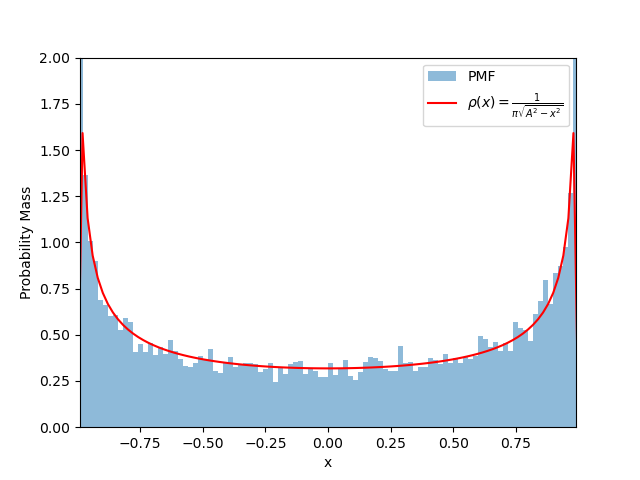
\includegraphics[width=\textwidth]{./chapters/graphs_ch1/1_13_1.png} Experimental results agree with analytical expression.}
\\ \\
\exercise{1.14}{
	Let $P_{ab}(t)$ be the probability of finding the particle in the range $(a < x < b)$, at time t. 
	\begin{itemize}
		\item Show that $$\derivative{P_{ab}}{t} = J(a,t) - J(b,t)$$ where $$J(x,t) \equiv \frac{i \hbar}{2m} \Biggl(\Psi \pdv{\Psi^*}{x}-\Psi^*\pdv{\Psi}{x}\Biggr) $$ What are the units of $J(x,t)$? Comment: $J$ is called the probability current, because it tells you the rate at which probability is ``flowing'' past point $x$. If $P_{ab}(t)$ is increasing,
		 then the more probability is flowing into the region at one end than flows out the other.
		 \begin{flalign*}
			\derivative{P_{ab}}{t} &= \derivative{}{t}\int_a^b |\Psi^2|~dx = \int_a^b \pdv{\Psi^*\Psi}{t}~dx\\
			&= \int_a^b \pdv{\Psi}{t}\Psi^*+\Psi\pdv{\Psi^*}{t}~dx\\
			&= \frac{i \hbar}{2m}\Psi^*\pdv[2]{\Psi}{x}-\frac{i\hbar}{2m}\pdv[2]{\Psi^*}{x}~dx\\
			&= \frac{i\hbar}{2m}\int_a^b \pdv{\Psi^*}{x}\pdv{\Psi}{x}+\Psi^*\pdv[2]{\Psi}{x}-\pdv[2]{\Psi^*}{x}\Psi-\pdv{\Psi}{x}\pdv{\Psi^*}{x}~dx\\
			&= \frac{i\hbar}{2m}\int_a^b \pdv{\Bigl(\Psi^*\pdv{\Psi}{x}-\Psi^*\pdv{\Psi}{x}\Bigr)}{x}~dx\\
			&= \frac{i\hbar}{2m} \biggl( \Psi^*\pdv{\Psi}{b}-\Psi\pdv{\Psi^*}{b}\biggr)-\frac{i\hbar}{2m} \biggl( \Psi^*\pdv{\Psi}{a}-\Psi\pdv{\Psi^*}{a}\biggr)\\
			&=J(b,t)-J(a,t)
		 \end{flalign*}
		 Probabilities don't have a dimension, so then $J$ must have units of 1/time, or $s^{-1}$, since this is a change in probability per change in time. 
		 \item Find the probability current for the wave function to 1.9. 
		 \begin{flalign*}
			\Psi(x,t) &= \sqrt[4]{\frac{2am}{\pi \hbar}} e^{-a\frac{mx^2}{\hbar}-ait} = f(x)e^{-ait}\\
			\Psi\pdv{\Psi^*}{x} &= f(x)e^{-ait}\pdv{f(x)}{x}e^{ait} = f(x)\pdv{f(x)}{x} = \Psi^*\pdv{\Psi}{x}\\
			\therefore J(x,t) &= 0\\
		 \end{flalign*}
	\end{itemize}
	Thus, we see a net zero probability flow in and out of this region: the probability of finding particle at position $x$ is a constant over this region should we have probability current of 0.
}
